\section{Parameter estimation}\label{sec2}

In order to apply subspace methods for parameter estimation, an underlying model has to be utilized with well defined parameters. Exponentially damped sinusoidal $(EDS)$ is a very convenient model and widely utilized in different signal processing applications figure \ref{EDS}. Hereby the signal being detected in the sensing device is modeled as a superposition of damping signals at distinct frequencies contaminated with white Gaussian noise $(wgn)$ equation \ref{eq1}. These components accommodate the information regarding the tissue properties, therefore accurate estimation of the amplitude $a_{k}$, frequency $f_{k}$, phase $\phi_{k}$ and damping $d_{k}$ is very critical. The analysis is performed in the frequency domain.   

 
\begin{equation}\label{eq1}
y(t)=\sum_{k=1}^{K} a_{k}exp(j\phi_{k})exp(-d_{k}t+2\pi f_{k}t)\delta t+wgn
\end{equation}

Utilizing the estimated parameter, a modeled signal (EDS) is then employed for peaks of interest computation . Via subspace methods based on (total) least square approximation a best fit between the modeled and the original signal is computed. This will enable a good estimation of peaks closely spaced,as well as their amplitudes. 

Herein the main algorithm being introduced is outlined in \ref{Ap2} which fits the model either via least square (LS) or via total least square (TLS). Additionally prior knowledge of poles are also being incorporated in the algorithm for further increase of the accuracy of the estimation. In order to validate the robustness of the methods, wgn is superimposed to the water filtered signal and the estimated parameters are then compared to the wgn free signal. 


Contrary to LS solution which introduces higher bias and inconsistency, TLS methods introduce an asymptotically bias compare to the ground truth solution \cite{7}. The known poles will enable the orthogonal projection of the data via QR decomposition whereby it will remove the known part \ref{Ap3}. 

In figure \ref{Nadya1} are the spectra of the reconstruction signal from the noise free signal respectively to the three methods. Whereas on the figure \ref{Nadya2} there are the spectra of the reconstructed signal from the noisy signal for respective method. 

The performance of each method is outlined in the table \ref{Nadya3}. The first row corresponds to the absolute mean value of the difference between the original and the fitted signal $\Delta=Signal-Fitted$. Herein there is a clear evidence that the mean value will increase for the same method from the pure to the noisy signal. This is the effect of the noise contamination which will worsen the performance of the method. The noise impact is also noted in the variance of $\Delta$ where the variability increases with a small factor in the noisy signal case. 

In case of method comparison, root-mean-square-error (RMSE) has been chosen as a good indicator. In the figure \ref{Nadya4} HSVD curve on average tends to stay above the other models. Thereby indicating a higher bias incorporated into the estimation. On the other hand, $HTLS_{_}$$PK_{_}$$FD$ outperforms HTLS based on the same graph in figure \ref{Nadya4}. Herein the RMSE tends to oscillate significantly for high level of noise and stabilizes the signal level significantly higher. However, on average the error introduced by $HTLS_{_}$$PK_{_}$$FD$ sits on lower values as compared to the HTLS case and HSVD.

The residue signal for each estimation is plotted in the figure \ref{Nadya5}, whereas the individual component superimposed together for the modeled signal are in the section \ref{Nadya6}. The estimated parameter including  amplitude, frequency, phase and damping via respective method are listed in the section \ref{Nadya7}.

\begin{figure}[!htbp]
\minipage{0.5\textwidth}%
\centering
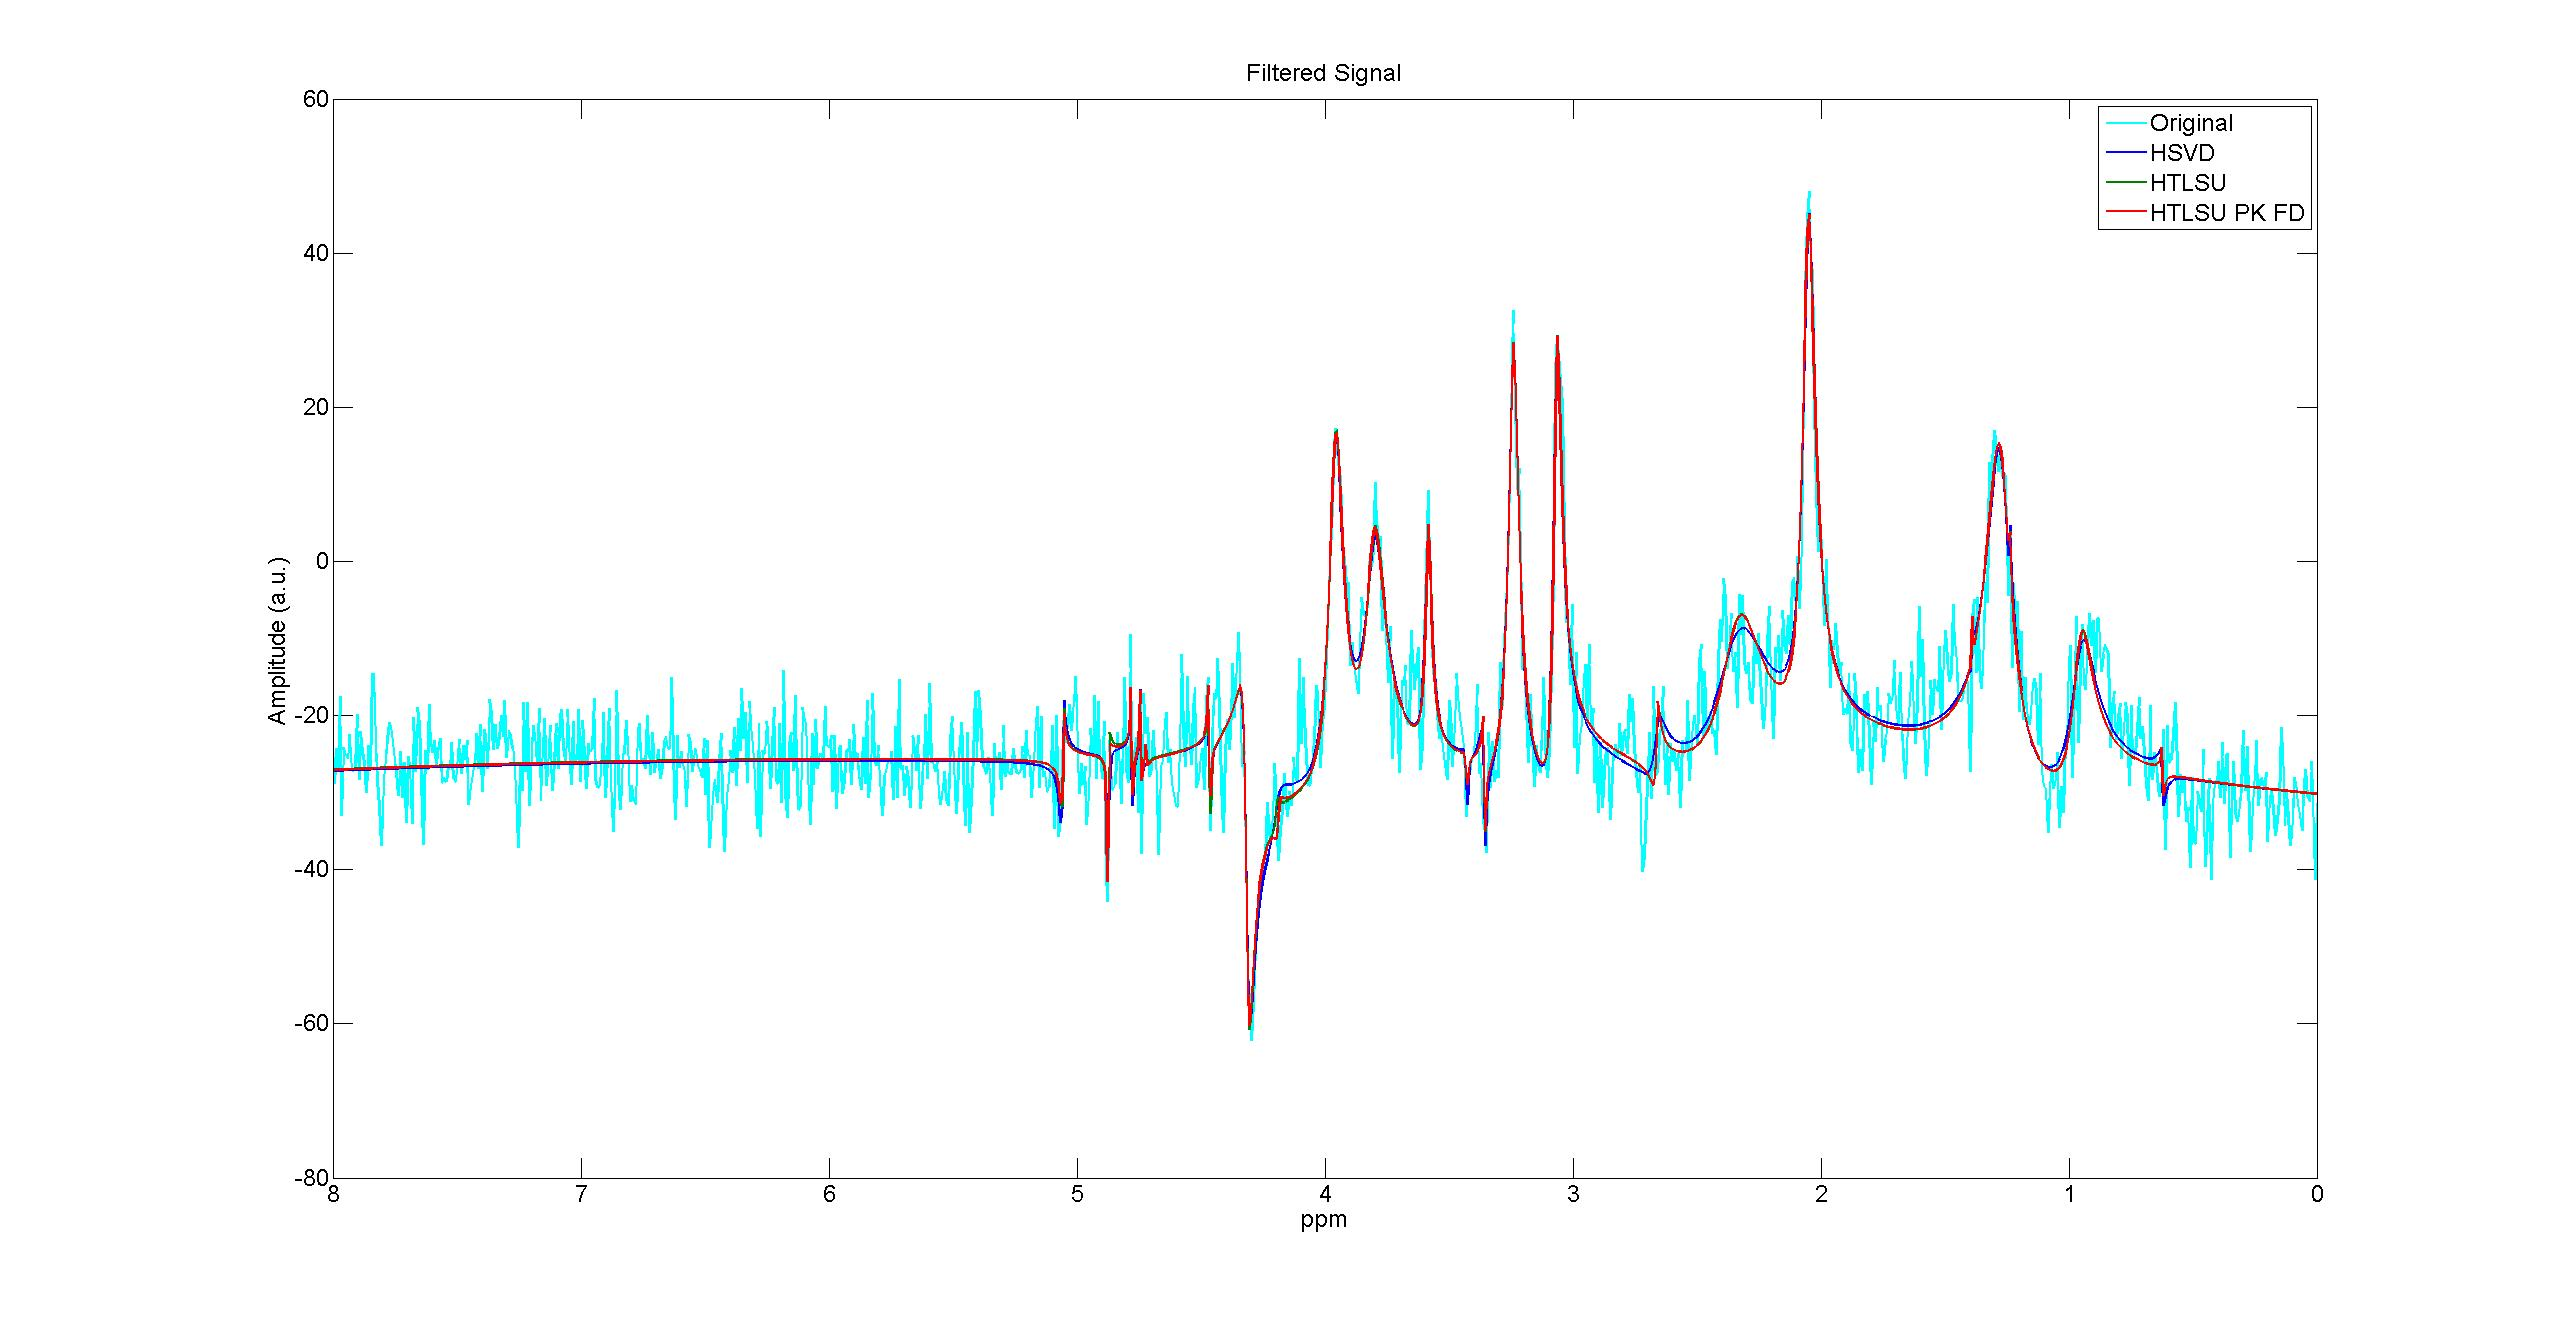
\includegraphics[width=1\textwidth]{114.jpg}
\subcaption{Filtered Signal}\label{Nadya1}
\endminipage\hfill
\minipage{0.5\textwidth}%
\centering
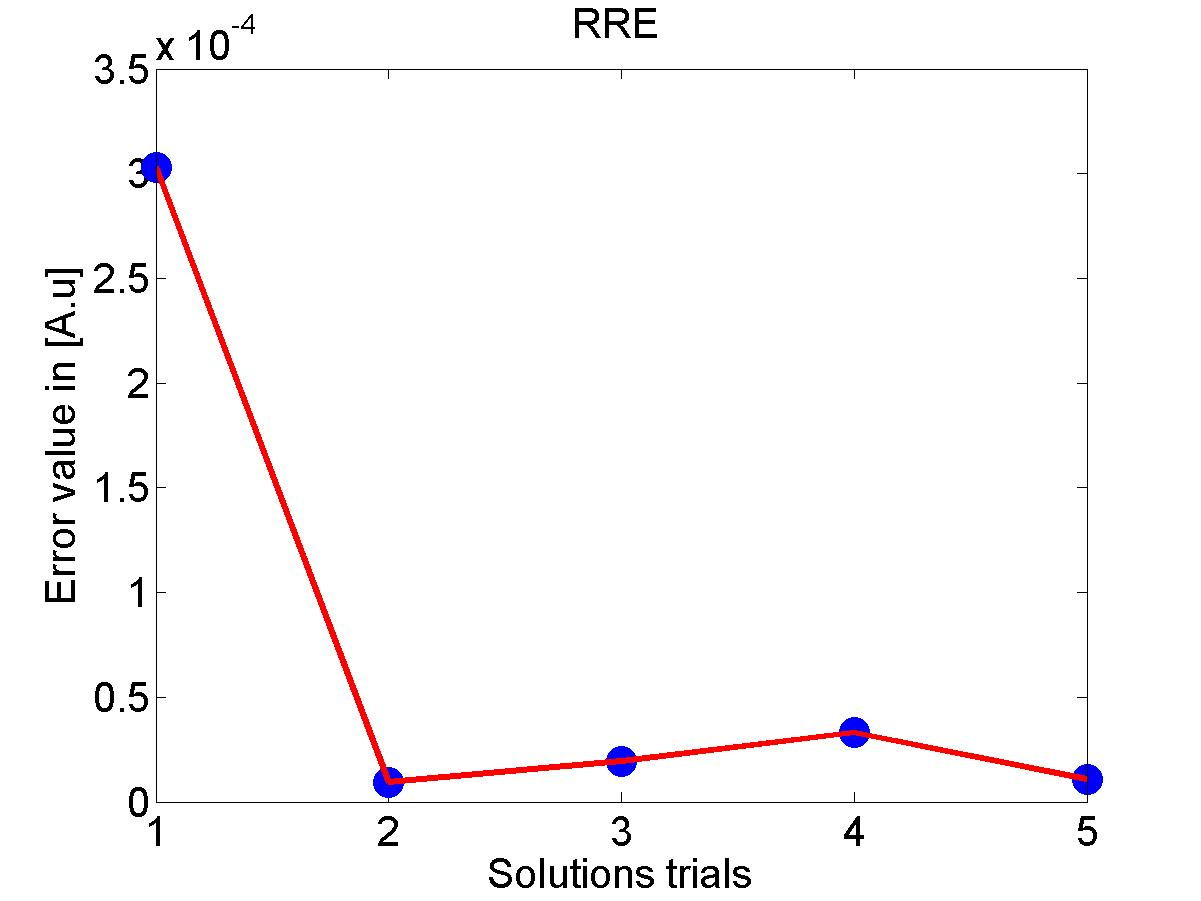
\includegraphics[width=1\textwidth]{115.jpg}\\
\subcaption{Noisy Signal}\label{Nadya2}
\endminipage\hfill
\caption{Reconstruction Outcome}
\end{figure}


\begin{figure}[!htbp]
\centering
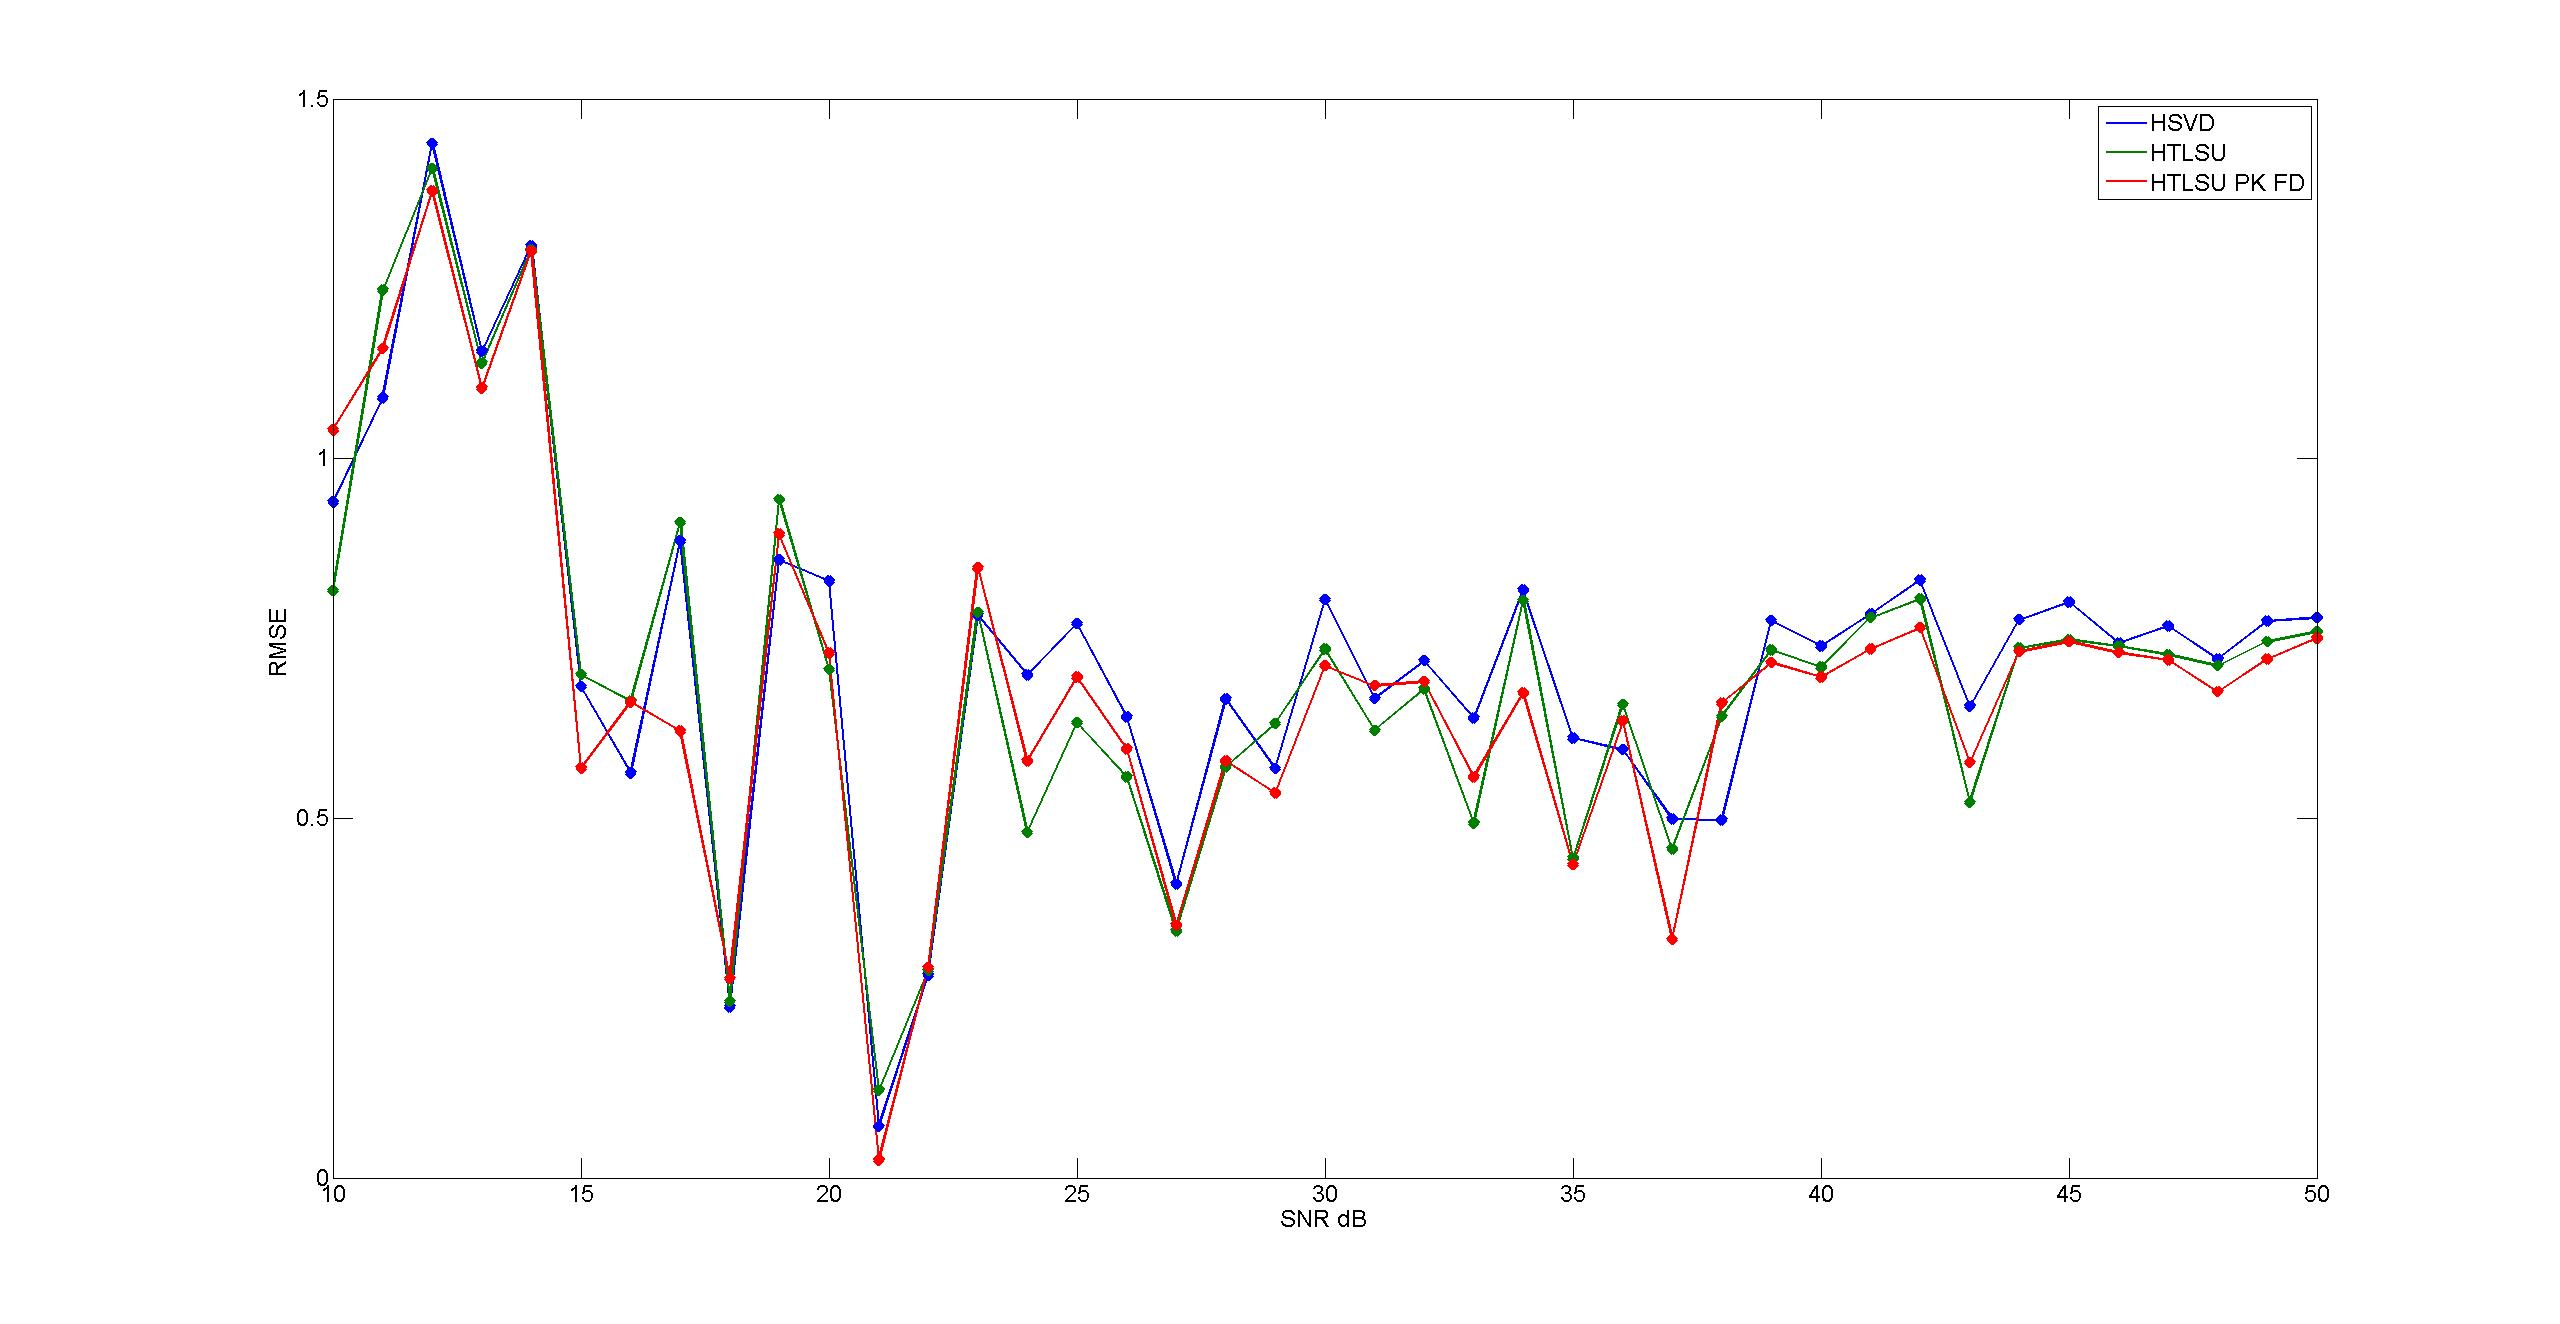
\includegraphics[width=0.7\textwidth]{RMSE.jpg}
\caption{Reconstruction Outcome}\label{Nadya4}
\end{figure}


 \begin{table}[!htbp]
\centering
\caption{Fitted performance}\label{Nadya3}

\begin{tabular}{c c c c c c c} 
\hline 

\input{Textfiles/5.txt}  

\hline 
\end{tabular}
\end{table}
 

\subsection{Subspace methods for parameter estimation}

\begin{itemize}
 
 \item In subspace method it is very hard to incorporate prior knowledge of the parameters to be estimated. However, in \cite{7} and \cite{8} the algorithm is proposed as an extension of HTLS capable of accommodating prior knowledge in the computation. It will increase the accuracy together with the resolution. Whereby it will facilitate the estimation of closed spaced peaks in the NMR spectrum with values very close to the Cramer-Rao (CR) lower bounds. The reason why the CR bounds became smaller is due to the non-zero mutual uncertainty of the parameters to be estimated. A further investigation is introduced in \ref{A2}.
 
 \item Subspace methods on the other hand are very robust framework. On other word it is a well-posed problem solution. It means that the solution exist and it is unique, nevertheless the solution is very sensitive to the initial conditions \cite{9}.
 
 \item Additionally the subspace methods are not iterative methods as compared to other optimisation based existing methods.Herein there is no cost function to be iteratively minimized, consequently the reproduction of data is ensured\cite{10}. The time complexity is much lower compare to optimisation based methods.
 
 \item Subspace based methods, however, don't suffer from local minimum. This is ensured from the lease square method wherein the best solution is outcomed. 

\item The user capability to initialize the parameters of the subspace methods is very important. In case of MRS signal the number of peaks are visually estimated. This restricts the method from being fully automatized. 

\item Furthermore, subspace methods are capable for parameter estimation of multiple different signals at the same time via the extension of the existing HTLS based algorithms\cite{10}. Consequently big data could be processed simultaneously instead of an iteration over single signal in the optimization case.


\end{itemize}



\newpage








